%!TEX root = ../../master.tex
\section*{Blog}

A blog has been created to share the progress of the project along with a source for the course in terms of guides explaining how to set up, e.g. Spring Cloud Zuul or similar. This guide contains a total of 18 blog posts about how to setup a Raspberry Pi Kubernetes Cluster, How to use Spring Boot, Configurations for various Kubernetes related topics, etc.

\renewcommand*{\arraystretch}{2}
\begin{tabular}{p{7cm}p{7cm}}
\centering
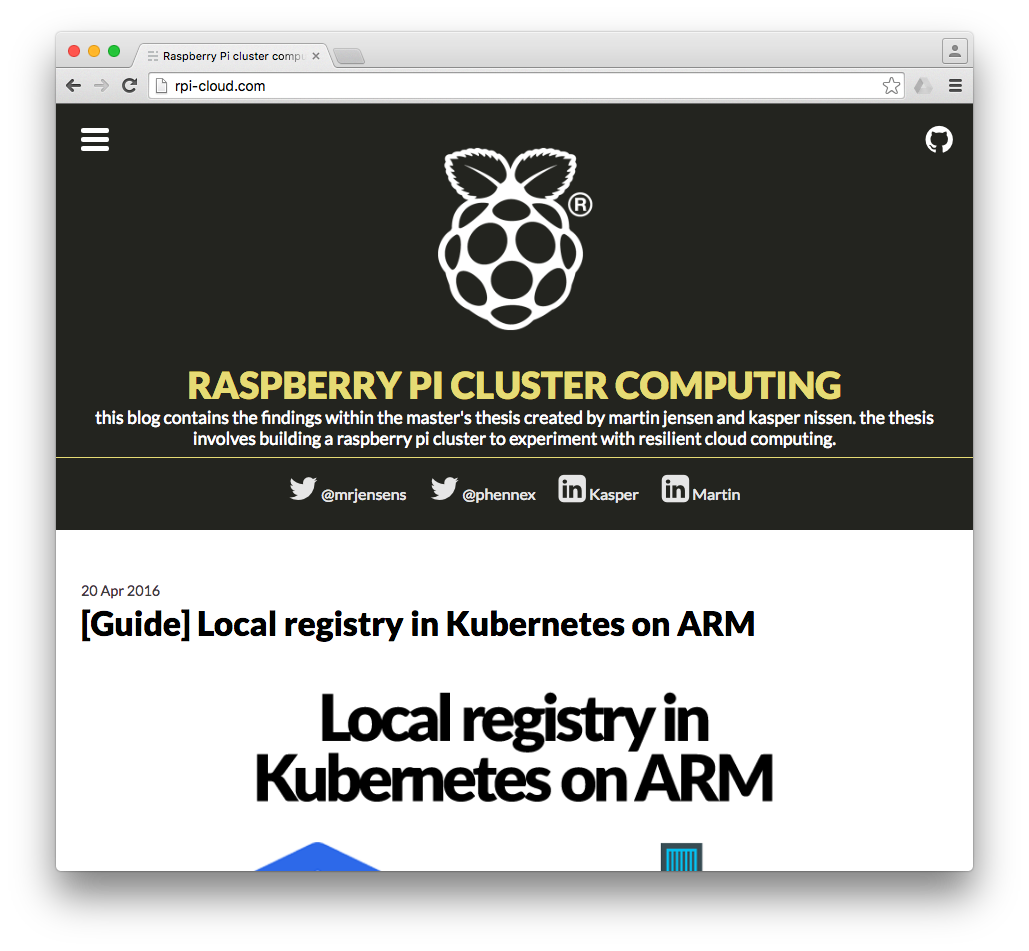
\includegraphics[align=t,width=7cm]{figures/blog/blog4} & 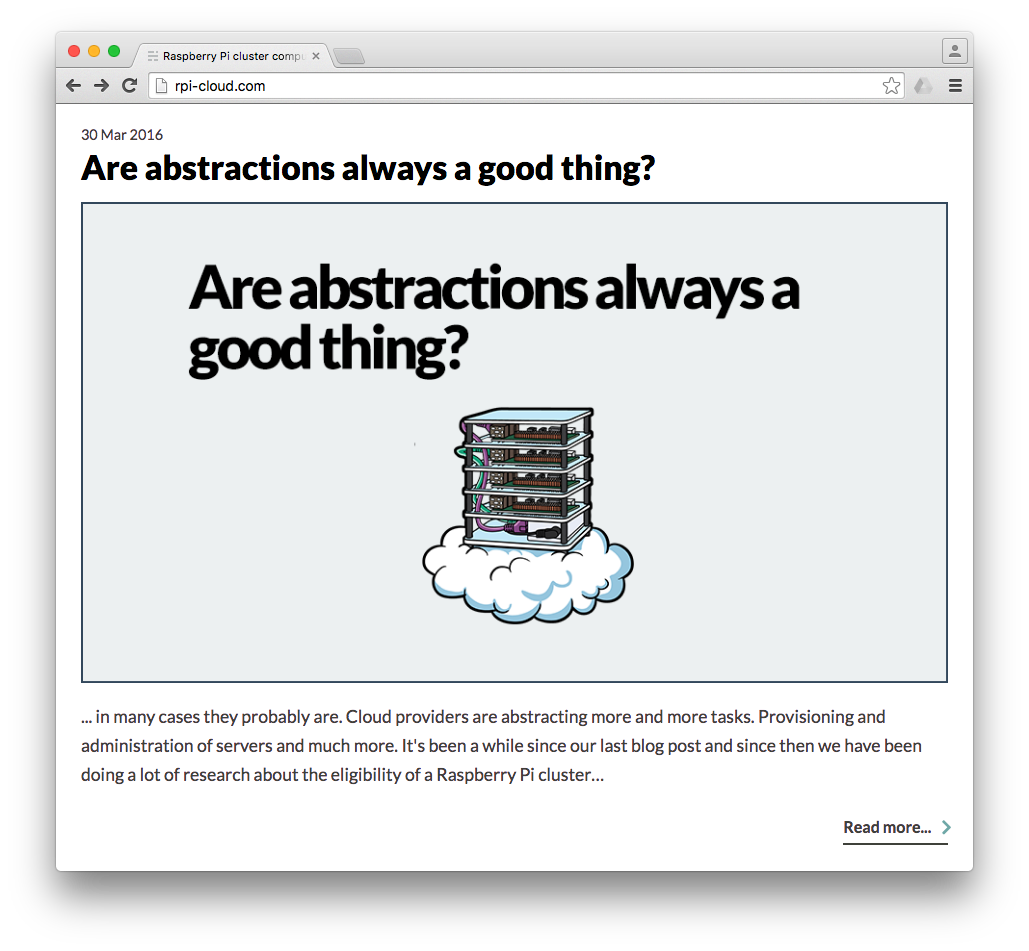
\includegraphics[align=t,width=7cm]{figures/blog/blog1} \\
\end{tabular}

\newpage
\noindent\begin{tabular}{p{7cm}p{7cm}}
\centering
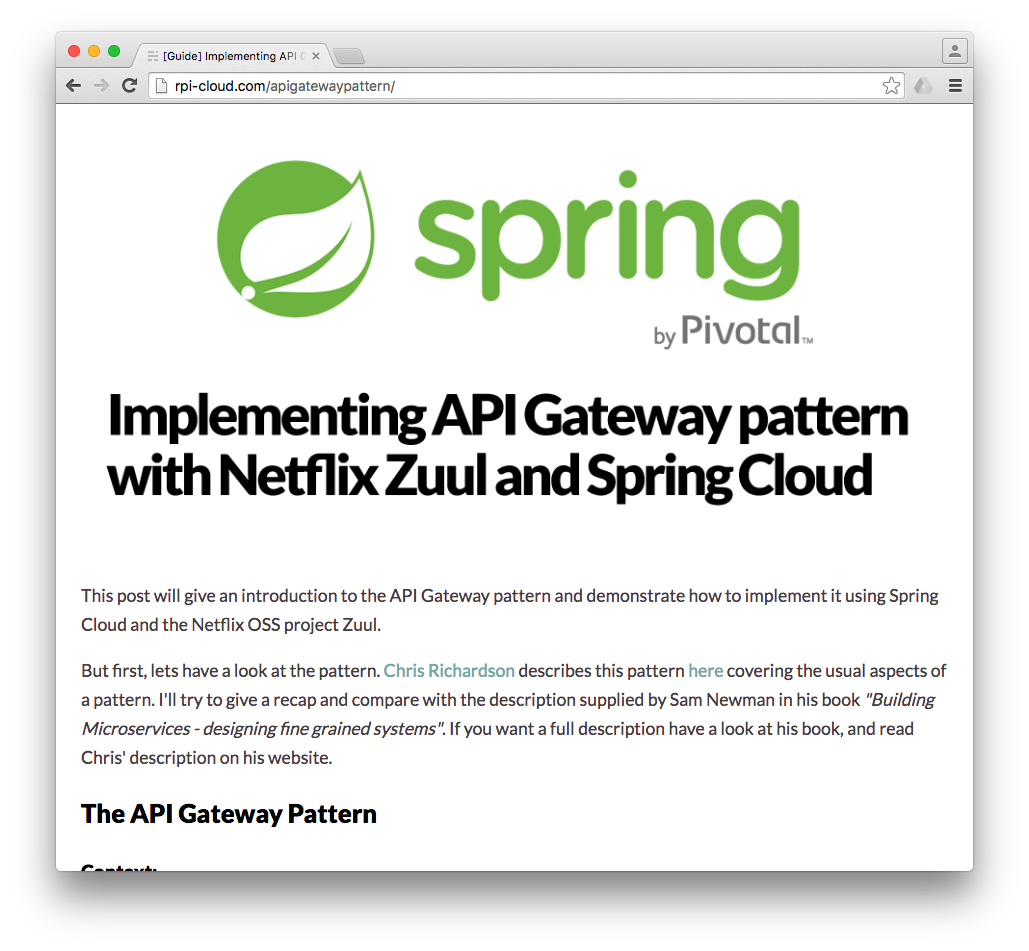
\includegraphics[align=t,width=7cm]{figures/blog/blog2} & 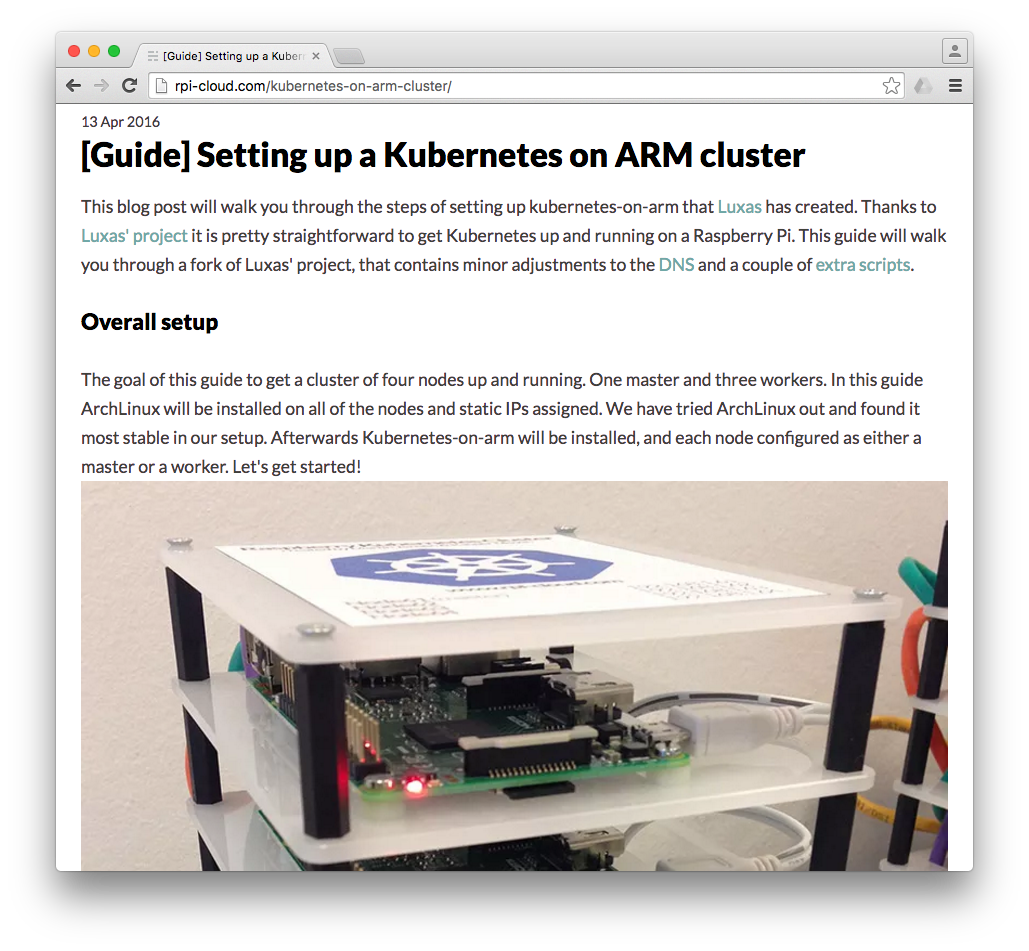
\includegraphics[align=t,width=7cm]{figures/blog/blog3} \\  

\end{tabular}